%% ------------------------------------------------------------------------- %%
\chapter{Experimentos}
\label{cap:exp}
\section{Descrição}


Os experimentos consistiram em medir a acurácia da IFT ao separar objeto e fundo de uma imagem. Os experimentos foram rodados para o banco de imagens públicas do grabcut que contém 50 imagens. 
Pode-se considerar que foram feitos duas classes de rotinas principais:

\begin{itemize}
\item IFT sobre uma imagem bruta, sem pré-processamento em regioes (nível de pixels).
\item IFT sobre regioes geradas pelo método SLIC, com 100, 400, 900 e 1600 superpixels.
\end{itemize}



\begin{figure}[!h]
\begin{center}
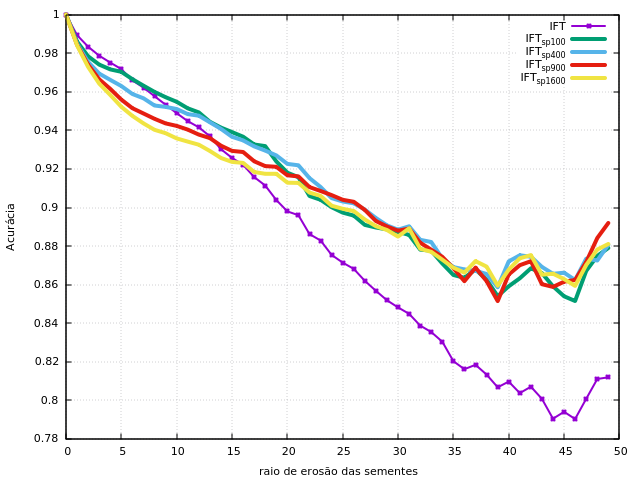
\includegraphics[width=14cm]{figuras/resultados}
\caption{\label{fig:resultados} resultados dos experimentos}
\end{center}
\end{figure}
